% \textbf{\underline{OZ 4 - De wet van Ampère en de wet van Biot-Savart - Oefening 1:}}
% \vspace{0.5cm}

% Bepaal het magnetische veld in het centrum van de halve cirkel in Figuur 4.1 als je weet dat de straal van de cirkel 4,00 cm bedraagt, de rechte stukken tot oneindig verder lopen en er een stroom van 6,00 A door de draad loopt.

% \begin{figure}[H]
%     \centering
%     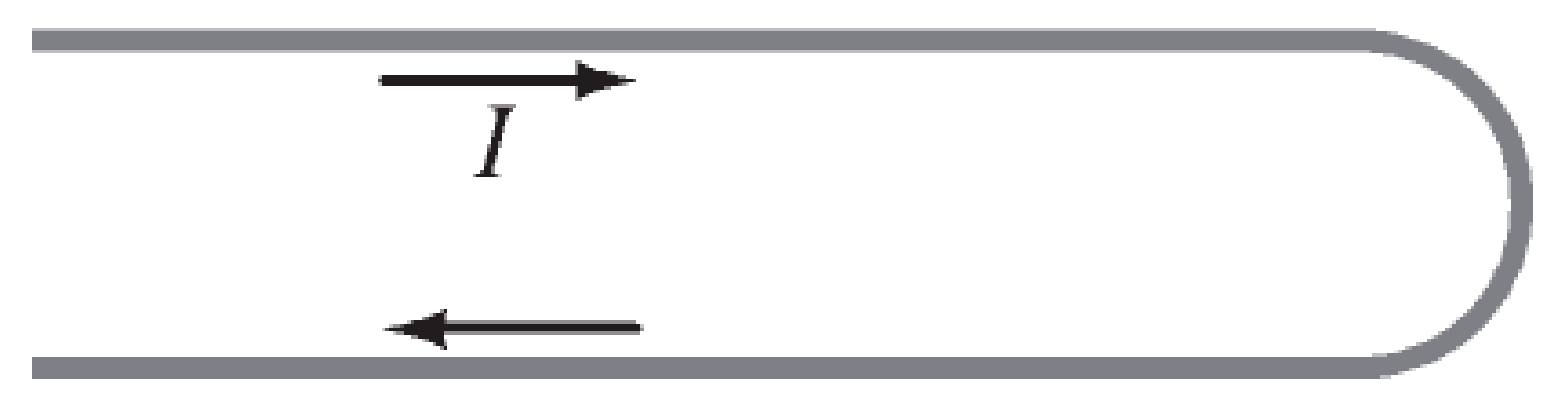
\includegraphics[width=4cm]{oz04/resources/oef-1-opgave.png}
    
%     \textbf{Figuur 4.1}
% \end{figure}

% \begin{description}[labelwidth=1.5cm, leftmargin=!]
%     \item[Geg. :]   $ r = 4,00 $ cm; $ I = 6,00 $ A;
%     \item[Gevr. :]  $ \vec{B} $;
%     \item[Opl. :]   Als we de 2 rechte stukken samen beschouwen als 1 oneindig lange geleider, kunnen we de hele oefening bekijken als een oneindig lange rechte geleider op afstand $ r $ en een demicirkel met straal $ r $.
    
%                     $ \vec{B}_{recht} = -\dfrac{\mu_0 I}{2 \pi r} \hat{k} $
                    
%                     \vspace{0.5cm}
    
%                     $ d\vec{B}_{demicirkel} = -k_m \dfrac{I d\vec{s} \times \hat{r}}{r^2} 
%                     = -k_m \dfrac{I d\theta}{r} \hat{k} $
                    
%                     \hspace{-0.57cm} $ \Leftrightarrow 
%                     \int_{0}^{\vec{B}_{demicirkel}}{d\vec{B}_{demicirkel}} = -\int_{0}^{\pi}{k_m \dfrac{I d\theta}{r}} \hat{k} $
                    
%                     \hspace{-0.57cm} $ \Leftrightarrow 
%                     \vec{B}_{demicirkel} = -k_m \dfrac{I \pi}{r} \hat{k} $
                    
%                     \vspace{0.5cm}
    
%                     $ \vec{B} = \vec{B}_{recht} + \vec{B}_{demicirkel} $
                    
%                     \hspace{0.27cm} $
%                     = -\dfrac{\mu_0 I}{2 \pi r} \hat{k} - k_m \dfrac{I \pi}{r} \hat{k} $
                    
%                     \hspace{0.27cm} $
%                     = -\dfrac{4 \pi \cdot 10^{-7} \cdot 6,00}{2 \pi \cdot 4,00 \cdot 10^{-2}} \hat{k} - 10^{-7} \dfrac{6,00 \cdot \pi}{4,00 \cdot 10^{-2}} \hat{k} $
                    
%                     \hspace{0.27cm} $
%                     = -77,12389 \hat{k} \ \mu$T
                    
%                     \hspace{0.27cm} $
%                     \approx -77,1 \hat{k} \ \mu$T
% \end{description}

% \vspace{1cm}